In tomographic medical imaging one of the main clinical and research needs is imaging information over the whole-body. Routine PET oncology applications require whole body coverage to detect and characterise the primary disease and any metastatic disease. This need for whole body coverage is not exclusive to oncology, many clinical and research applications can benefit from this type of information. In this chapter we will describe the main principles behind use of multi-bed PET acquisitions, their extension to dynamic imaging and our work in implementing and optimizing dynamic whole body acquisition protocols on the Signa PET/MR system. 

\subsection{WB PET}
The first suggestion and optimization work in extending the axial FOV of PET scans using multiple bed positions was by made by Dahlbom \textit{et al.}~\cite{Dahlbom1992}. This work was made on PET systems operated in 2D mode, where a bed displacement of approximately equal to the system A-FOV was used to increase the acquisition coverage (effective A-FOV). As systems became capable of acquiring in 3D mode, which offers increased sensitivity but result in axial varying sensitivity profiles, different strategies were needed for multi-bed acquisitions. The two methods suggested and developed are the \textit{Step and Shoot}(SS) and the \textit{Continuous Bed Motion}(CBM) aquisition method. 

\subsubsection{Step and Shoot}
The SS method makes use of multiple bed positions that are partially overlapped in the axial direction to increase the sensitivity of the acquisition at the edges of each beds FOV, by combining data of adjacent beds over the overlapping region as shown in figure~\ref{fig3_1:fullOverlap}. One way of treating such datasets is to reconstruct each bed individually, displace the reconstructed images according to their axial location and combine them using weighted averaging~\cite{Schubert1996}. This method has prevailed in clinical PET systems that use the SS acquisition method, as it does not require addition considerations in the reconstruction process of each bed and the combination of bed images can be performed post-reconstruction. Alternatively the axial displacement of each bed raw dataset can be performed during the projection and back-projection process in iterative reconstruction, which then directly results in the reconstruction of the whole-body image~\cite{Ross2004}. Use of the overlap data in iterative reconstruction can potentially result to improved noise characteristics at the overlapping regions, as the full sampled statistics over these regions are combined prior to each image update~\cite{Ross2004,Stute2014}. 
%
\begin{figure} [ht!]
\centering
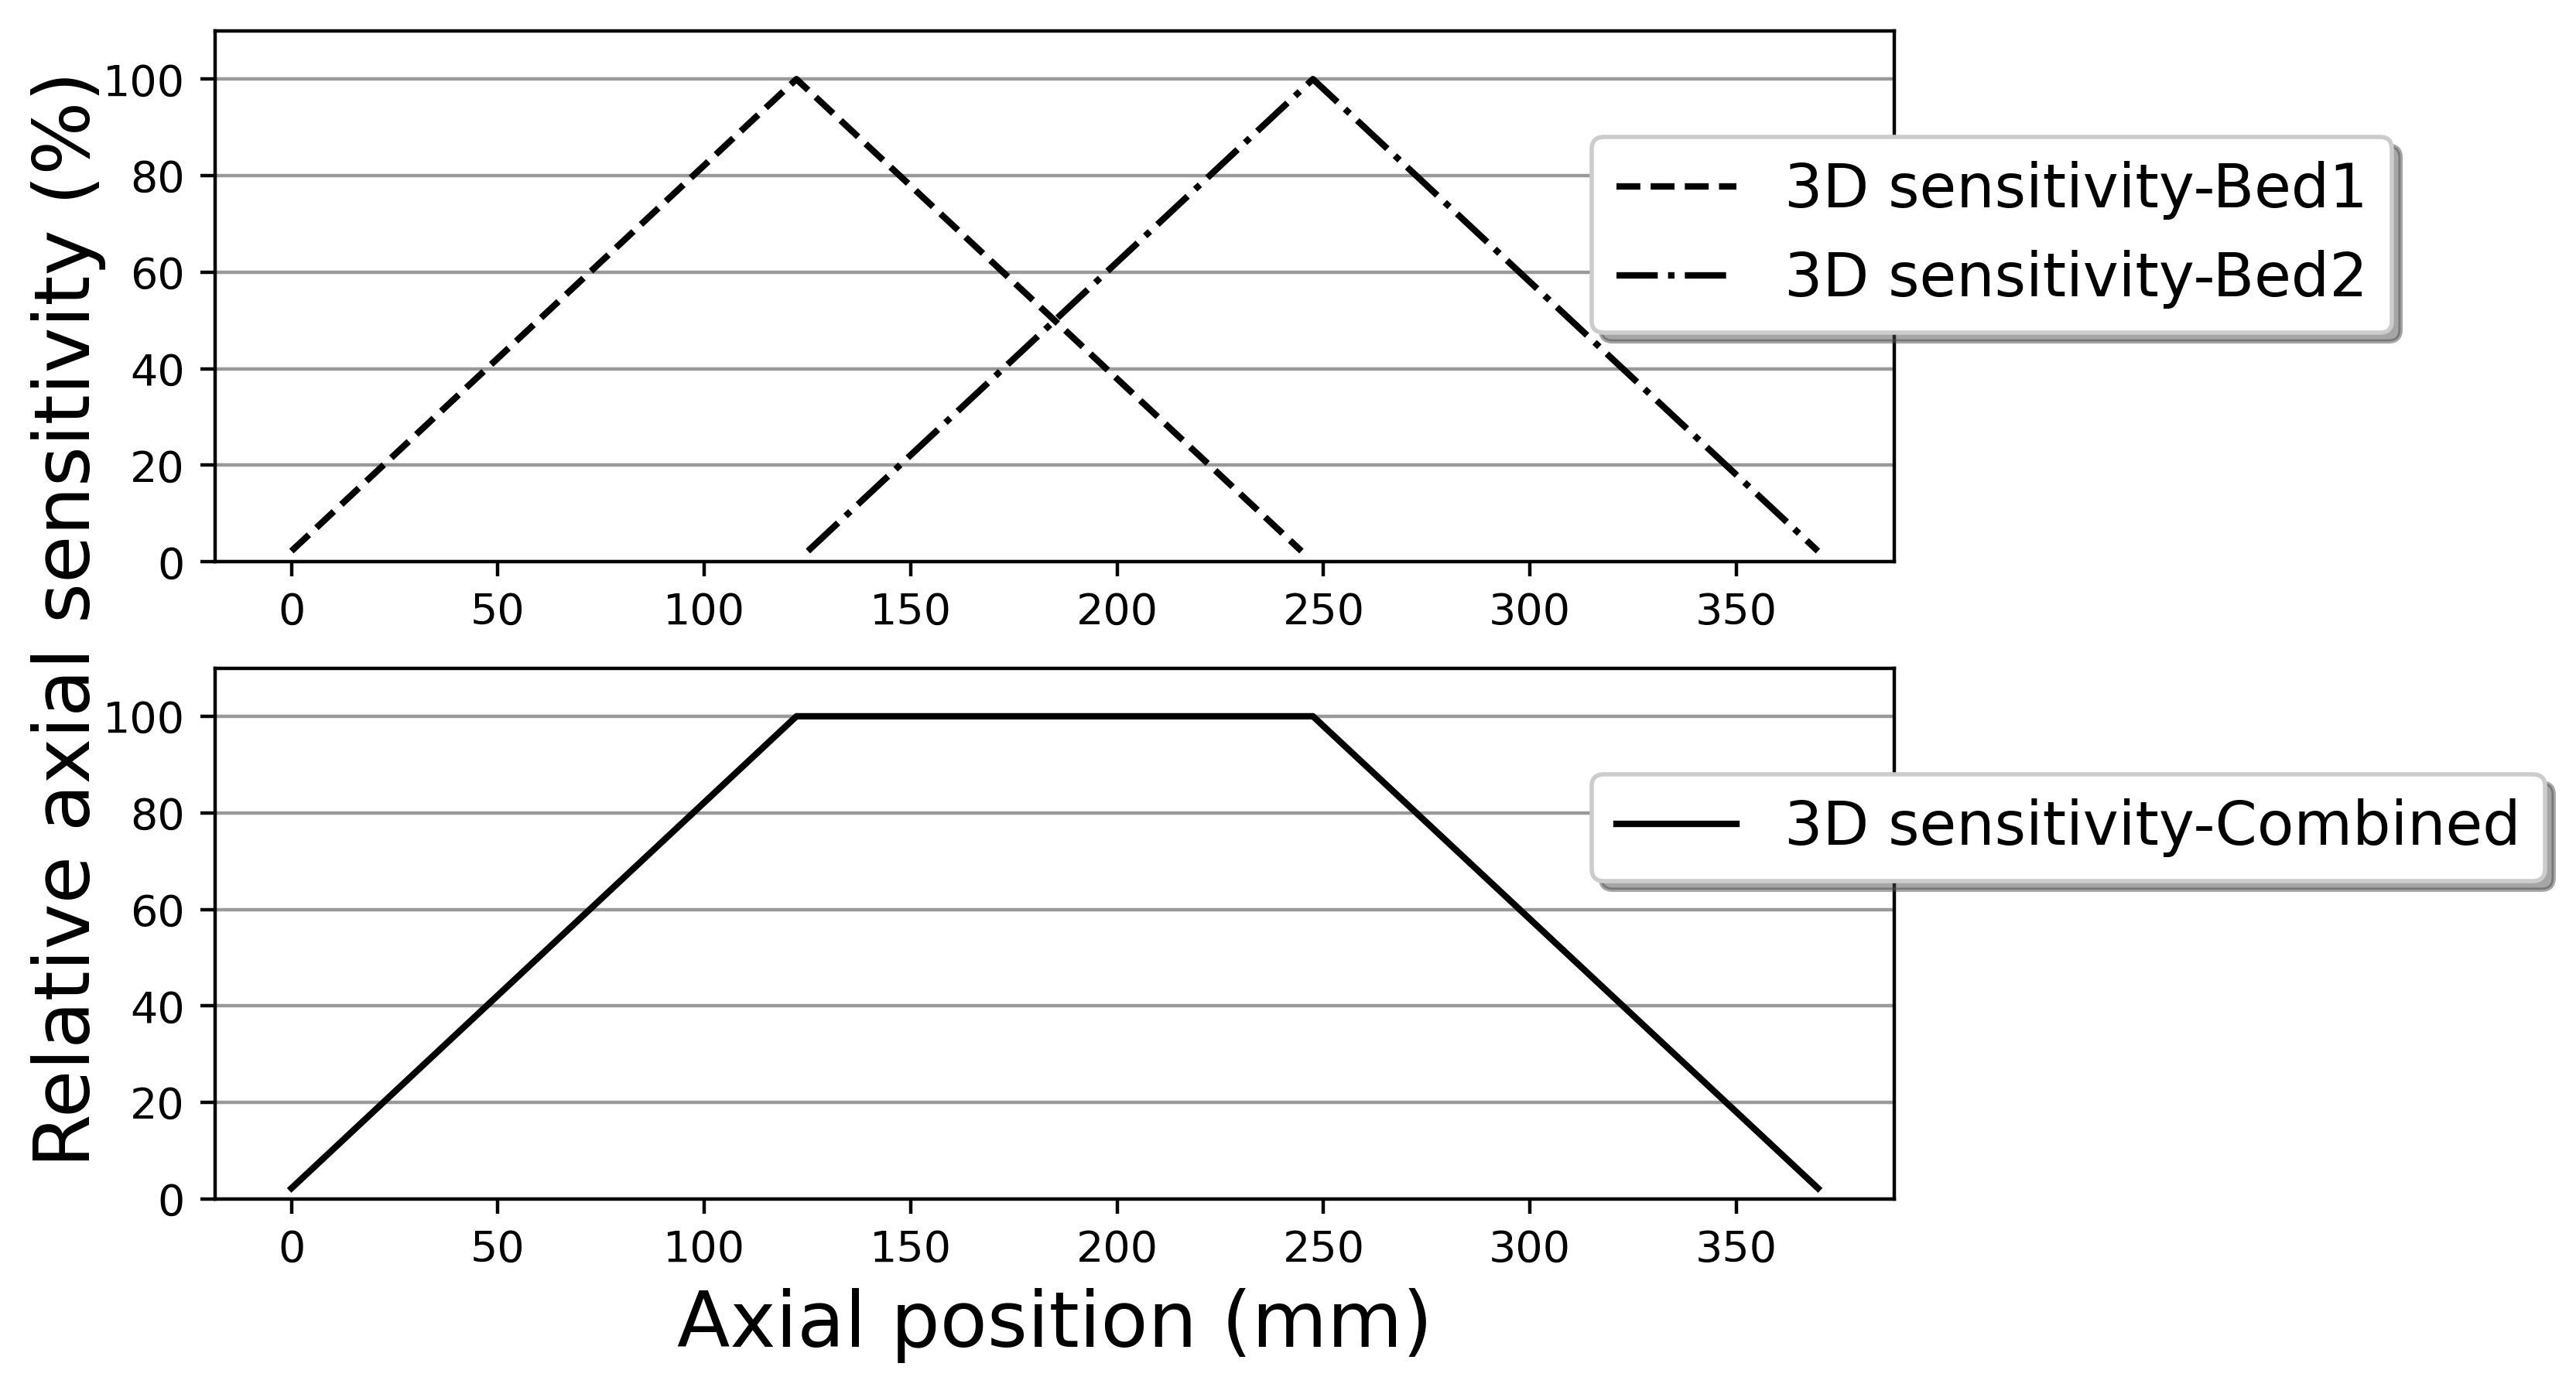
\includegraphics[scale=0.5,angle=0]{3_Results/3_1_DWB_Optimization/figures/SensitivityProfiles_fullOverlap.png}
\caption{Relative axial sensitivity of individual beds (top) and combined sensitivity profile (bottom) for approximately 50\% overlap.} 
%TODO: Add over-scan in the CBM D-WB protocols. 
\label{fig3_1:fullOverlap}
\end{figure}
%
The amount of overlap is a parameter to tune for some PET system. An example sensitivity profile for the Signa PET-MR system is shown. For a completely uniform axial sensitivity profile an overlap of 44 slices (\~50\% of A-FOV) is required, as shown in figure~\ref{fig3_1:fullOverlap}.
The amount of overlap used depends on the needs for uniformity in axial sensitivity and reconstructed image noise. This in term will also depend on the used reconstruction type and the activity distribution of the imaged subject~\cite{Schubert1996}. 
For standard clinical scanning at the Signa PET-MR an overlap of \~27\% is used to balance between sensitivity uniformity and scanning length or examination time. The trade-off is made to accommodate longer effective A-FOV in the same acquisition time or to reduce acquisition time by use of less bed positions to image the same scan length. Examples of three overlapping options are shown in figure~\ref{fig3_1:decreasingOverlap}.
%
\begin{figure} [ht!]
\centering
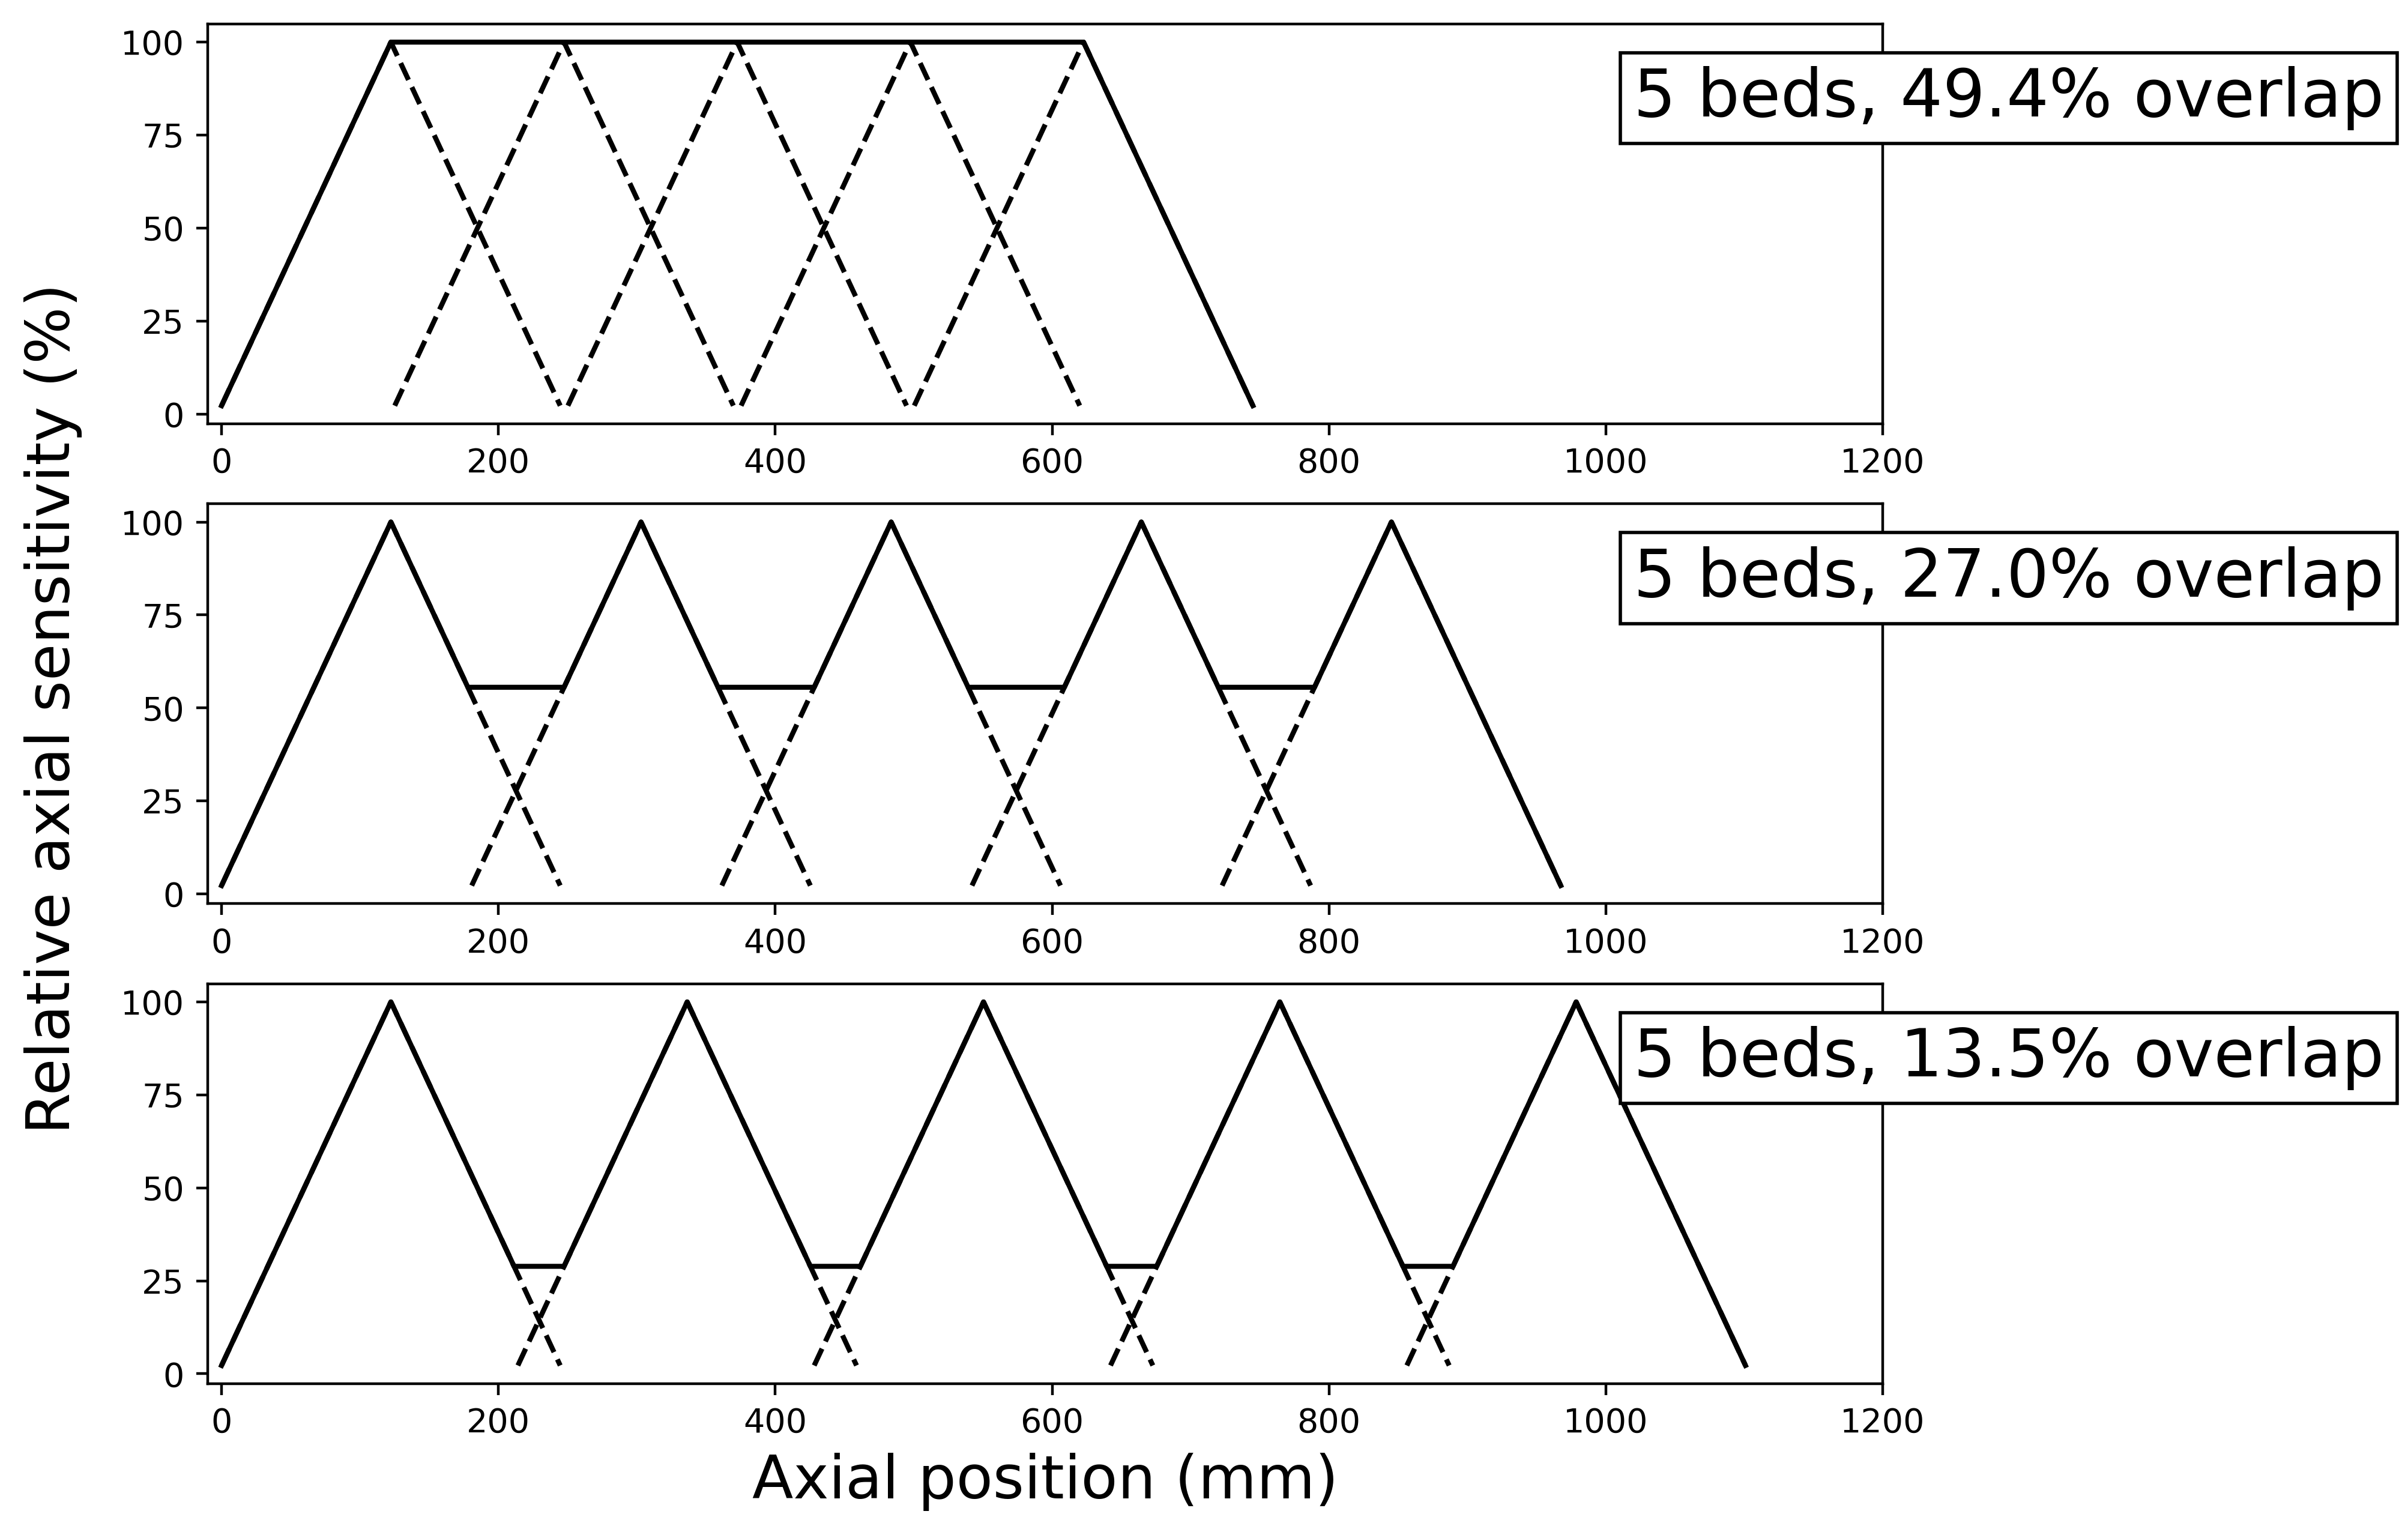
\includegraphics[scale=0.5,angle=0]{3_Results/3_1_DWB_Optimization/figures/SensitivityProfiles_3Options.png}
\caption{Relative axial sensitivity of 5 bed positions with decreasing overlap.} 
%TODO: Add over-scan in the CBM D-WB protocols. 
\label{fig3_1:decreasingOverlap}
\end{figure}
%
%
\begin{figure} [ht!]
\centering
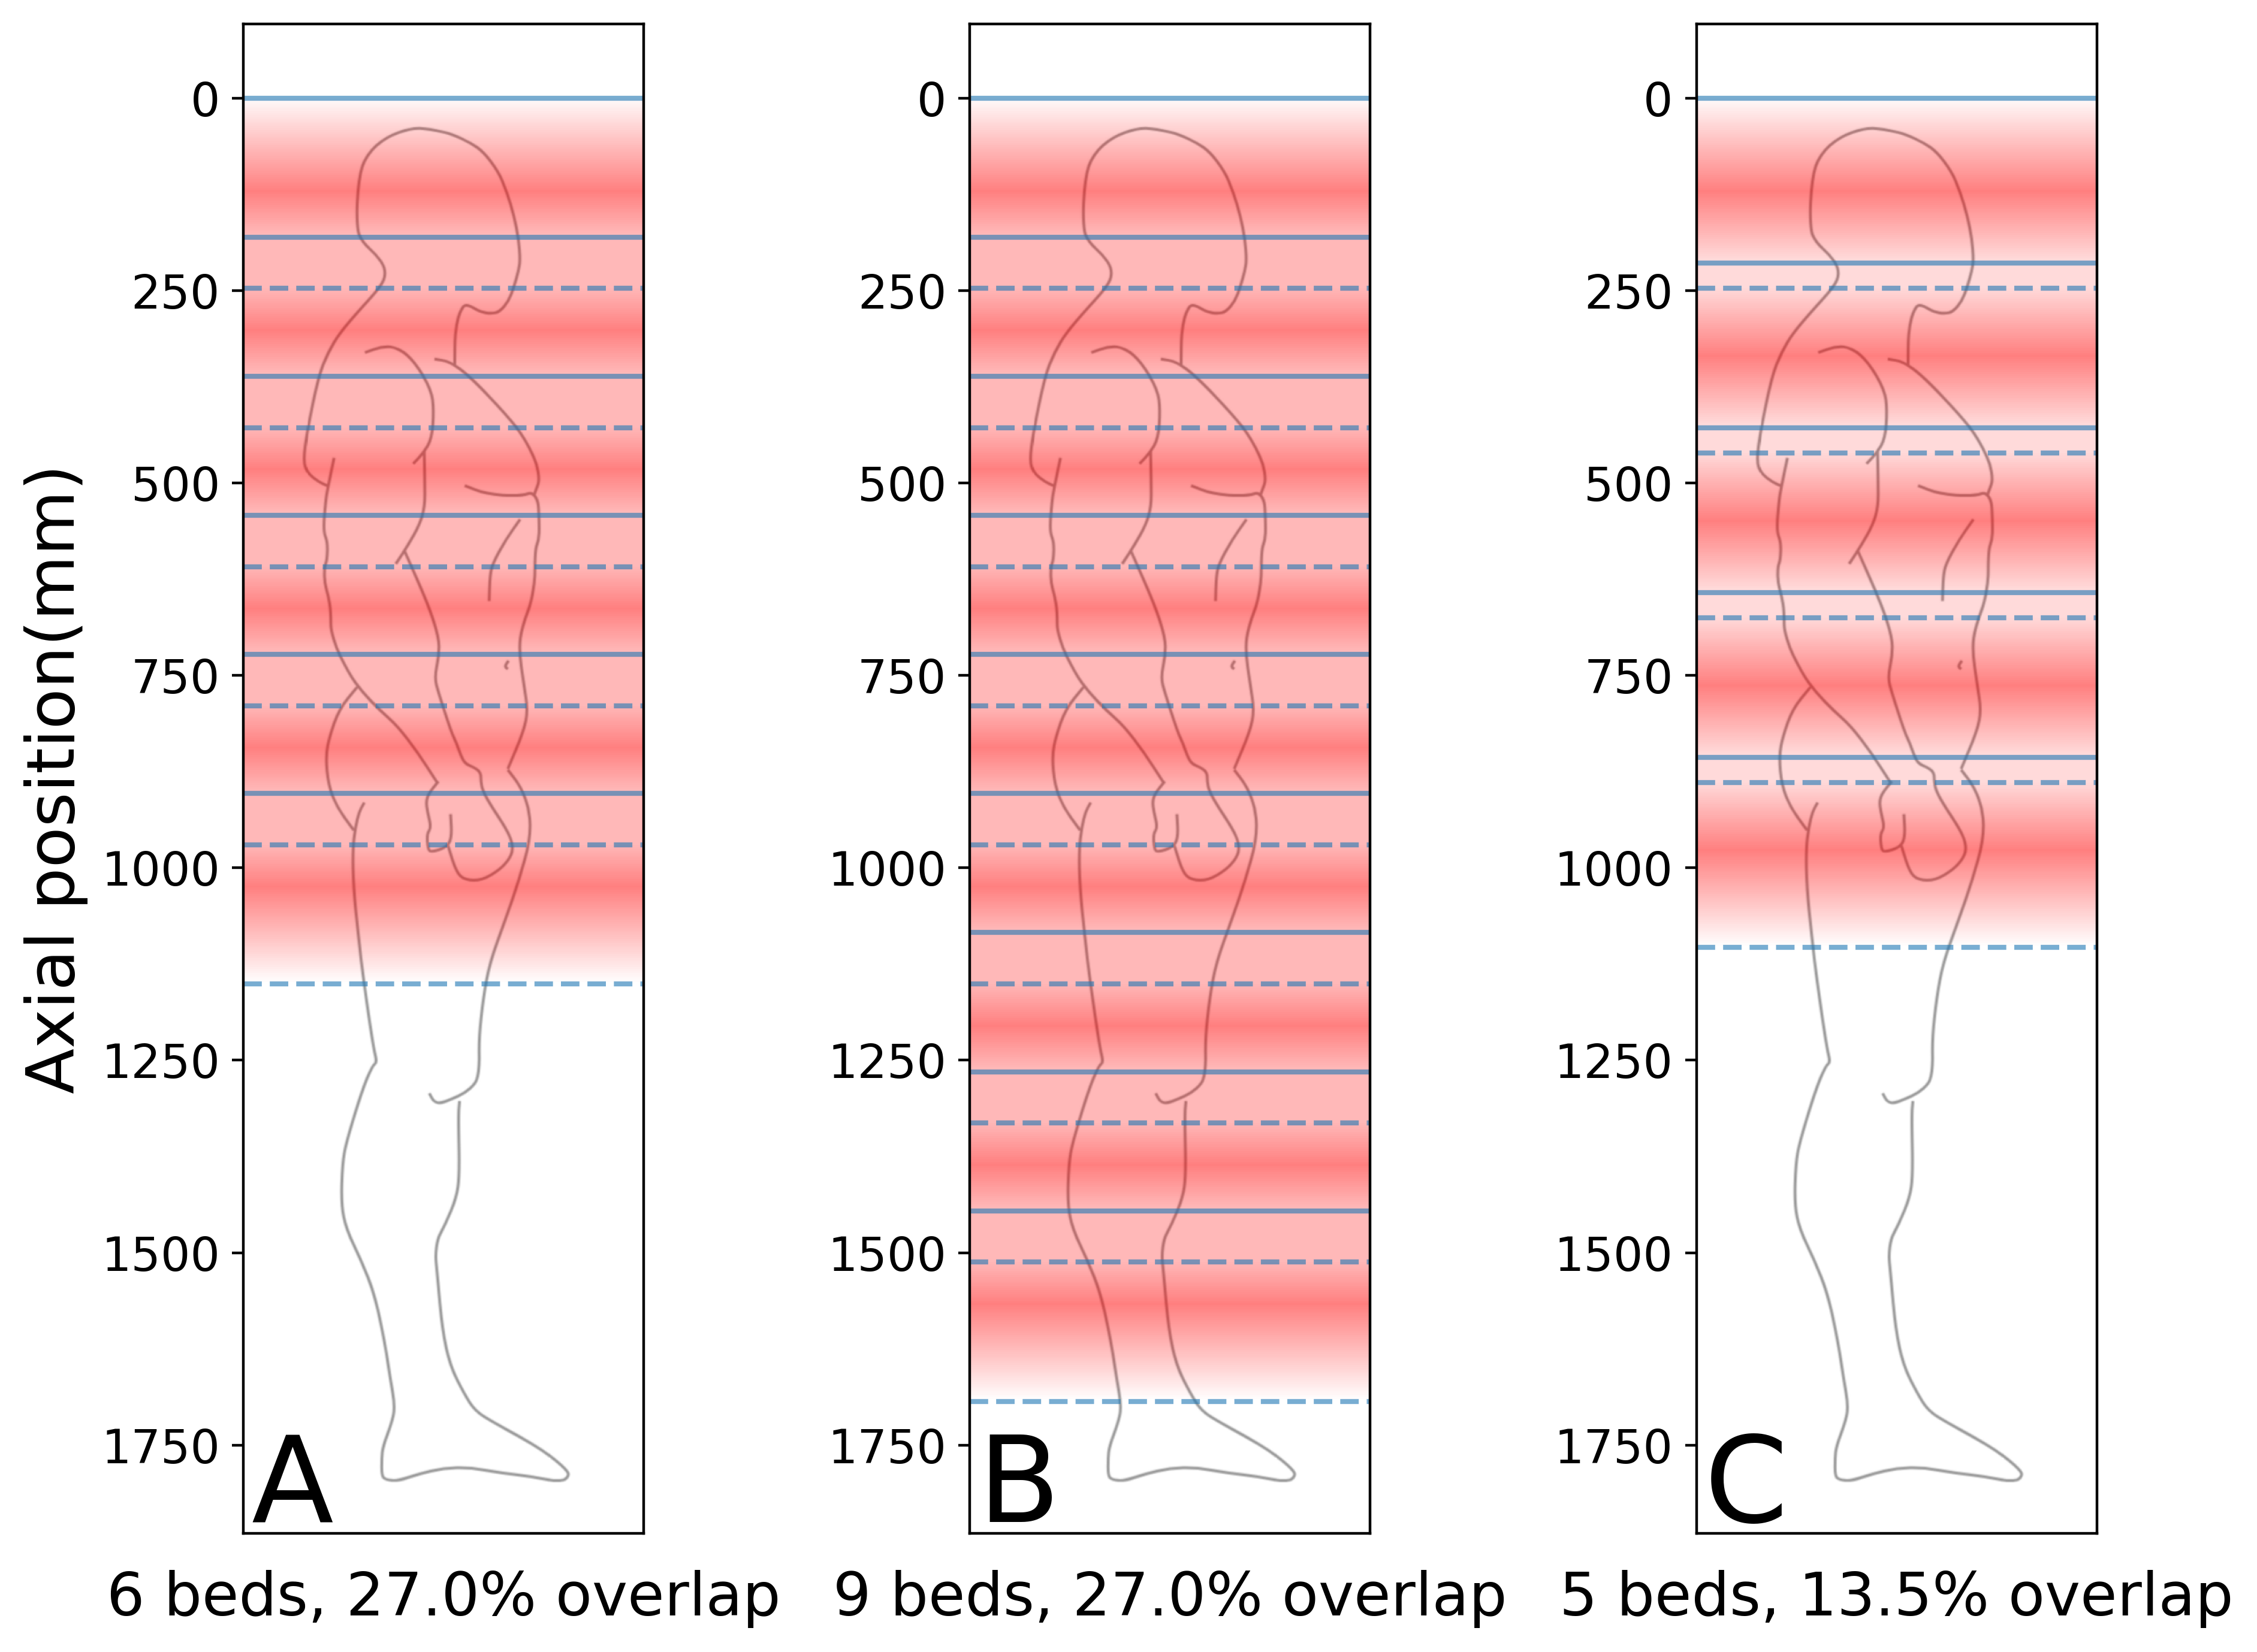
\includegraphics[scale=0.5,angle=0]{3_Results/3_1_DWB_Optimization/figures/SensitivityProfiles_overHuman.png}
\caption{Combinations of overlap and number of beds for static (A\&B) and dynamic whole-body imaging(C). Relative axial sensitivity is shown in shades of red, with bed start (\protect\tikz[baseline]{\protect\draw[line width=0.5mm] (0,.8ex)--++(1,0) ;}) and end (\protect\tikz[baseline]{\protect\draw[line width=0.5mm,densely dashed] (0,.8ex)--++(1,0) ;}) positions.} 
%TODO: Add over-scan in the CBM D-WB protocols. 
\label{fig3_1:BodyCoverage}
\end{figure}
%
For clinical scans an overlap of 27\% is used. Many WB applications actually require imaging of approximately half the length of the body, from head to thighs which requires 5 or 6 bed positions. When full body coverage is required the number is increased to 9 or 10 bed positions. In DWB acquisitions where fast scanning is crucial while maintaining a suitable body coverage, the overlap can be decreased as shown in option(C) in figure~\ref{fig3_1:BodyCoverage}. 

\subsubsection{Continuous Bed Motion}
Continuous Bed Motion was proposed as an extension of step and shoot acquisition performed in small steps, to provide uniform axial sensitivity profiles without the need of overlaps~\cite{Dahlbom2001,Brasse2002}. In CBM acquisitions the data are stored in list-mode while the bed is moving during the examination, with the data being sorted after or during the examination in sinograms (refereed as "chuncks") for reconstruction. The velocity of the bed movement can be adjusted depending on the amount of desired collected counts, similar to the acquisition time per bed in step and shoot. With newer systems the bed velocity can also be varied within an examination according to the needs and distribution of the imaged activity~\cite{Panin2014}. Beyond the technical gains, CBM protocols have been shown to also aid in patient comfort during~\cite{Schatka2016}. 

Many aspects of CBM acquisition can be beneficial over SS imaging, in particular for dynamic whole-body imaging~\cite{Karakatsanis2016}, but unfortunately this mode of acquisition is not available by the Signa PET-MR scanner.

\subsection{Dynamic WB PET}
